The PCCA kingdom has a world heritage site that everybody knows: The Triangular Cave.
Legend says there was an ancient civilization of triangles in the cave, and they left a powerful relic somewhere nobody knows.
One day, you find a mysterious triangular stone plate, and it turns out to be the legendary relic of the Holy Triangle!

The relic is divided into $n$ layers of small triangles, and the imprints enclose the small triangles.
You notice that some imprints have been charged with ancient power while others have not.
To fully empower the relic, you must restore it by making all the imprints charged.

However, you cannot charge the imprints directly.
Instead, you can replace the small triangle with the energy runestones you prepared beforehand.
An energy runestone is also in the shape of a triangle and can charge the imprints on the three sides of it once it is put onto the relic.

The figures below show examples of a relic before and after restoration:

\begin{figure}[h]
\center
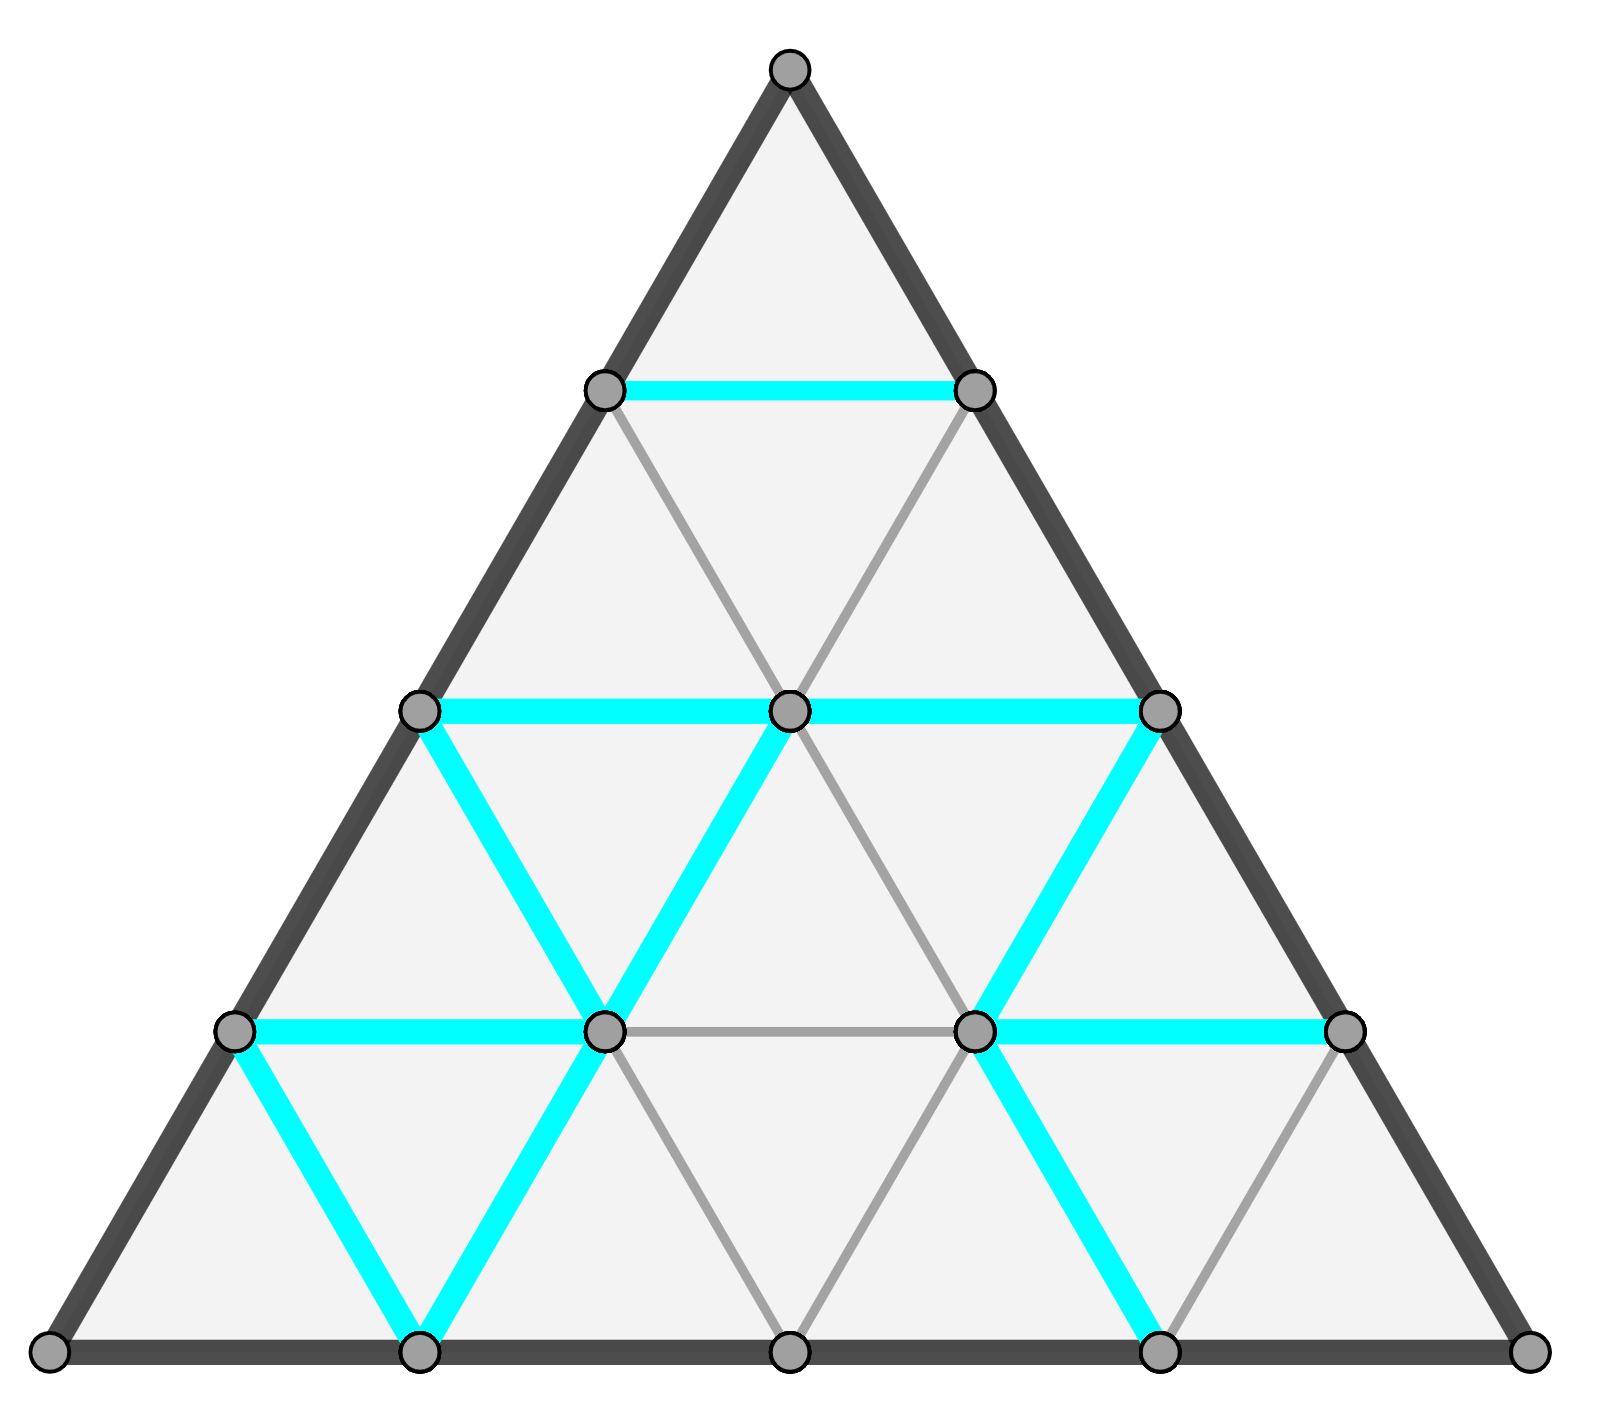
\includegraphics[width=0.35\textwidth]{image/relic1.png}
\caption{A partially charged relic before restoration. The blue edges are charged imprints and the grey edges are imprints not charged yet.}
\end{figure}
\begin{figure}[h]
\center
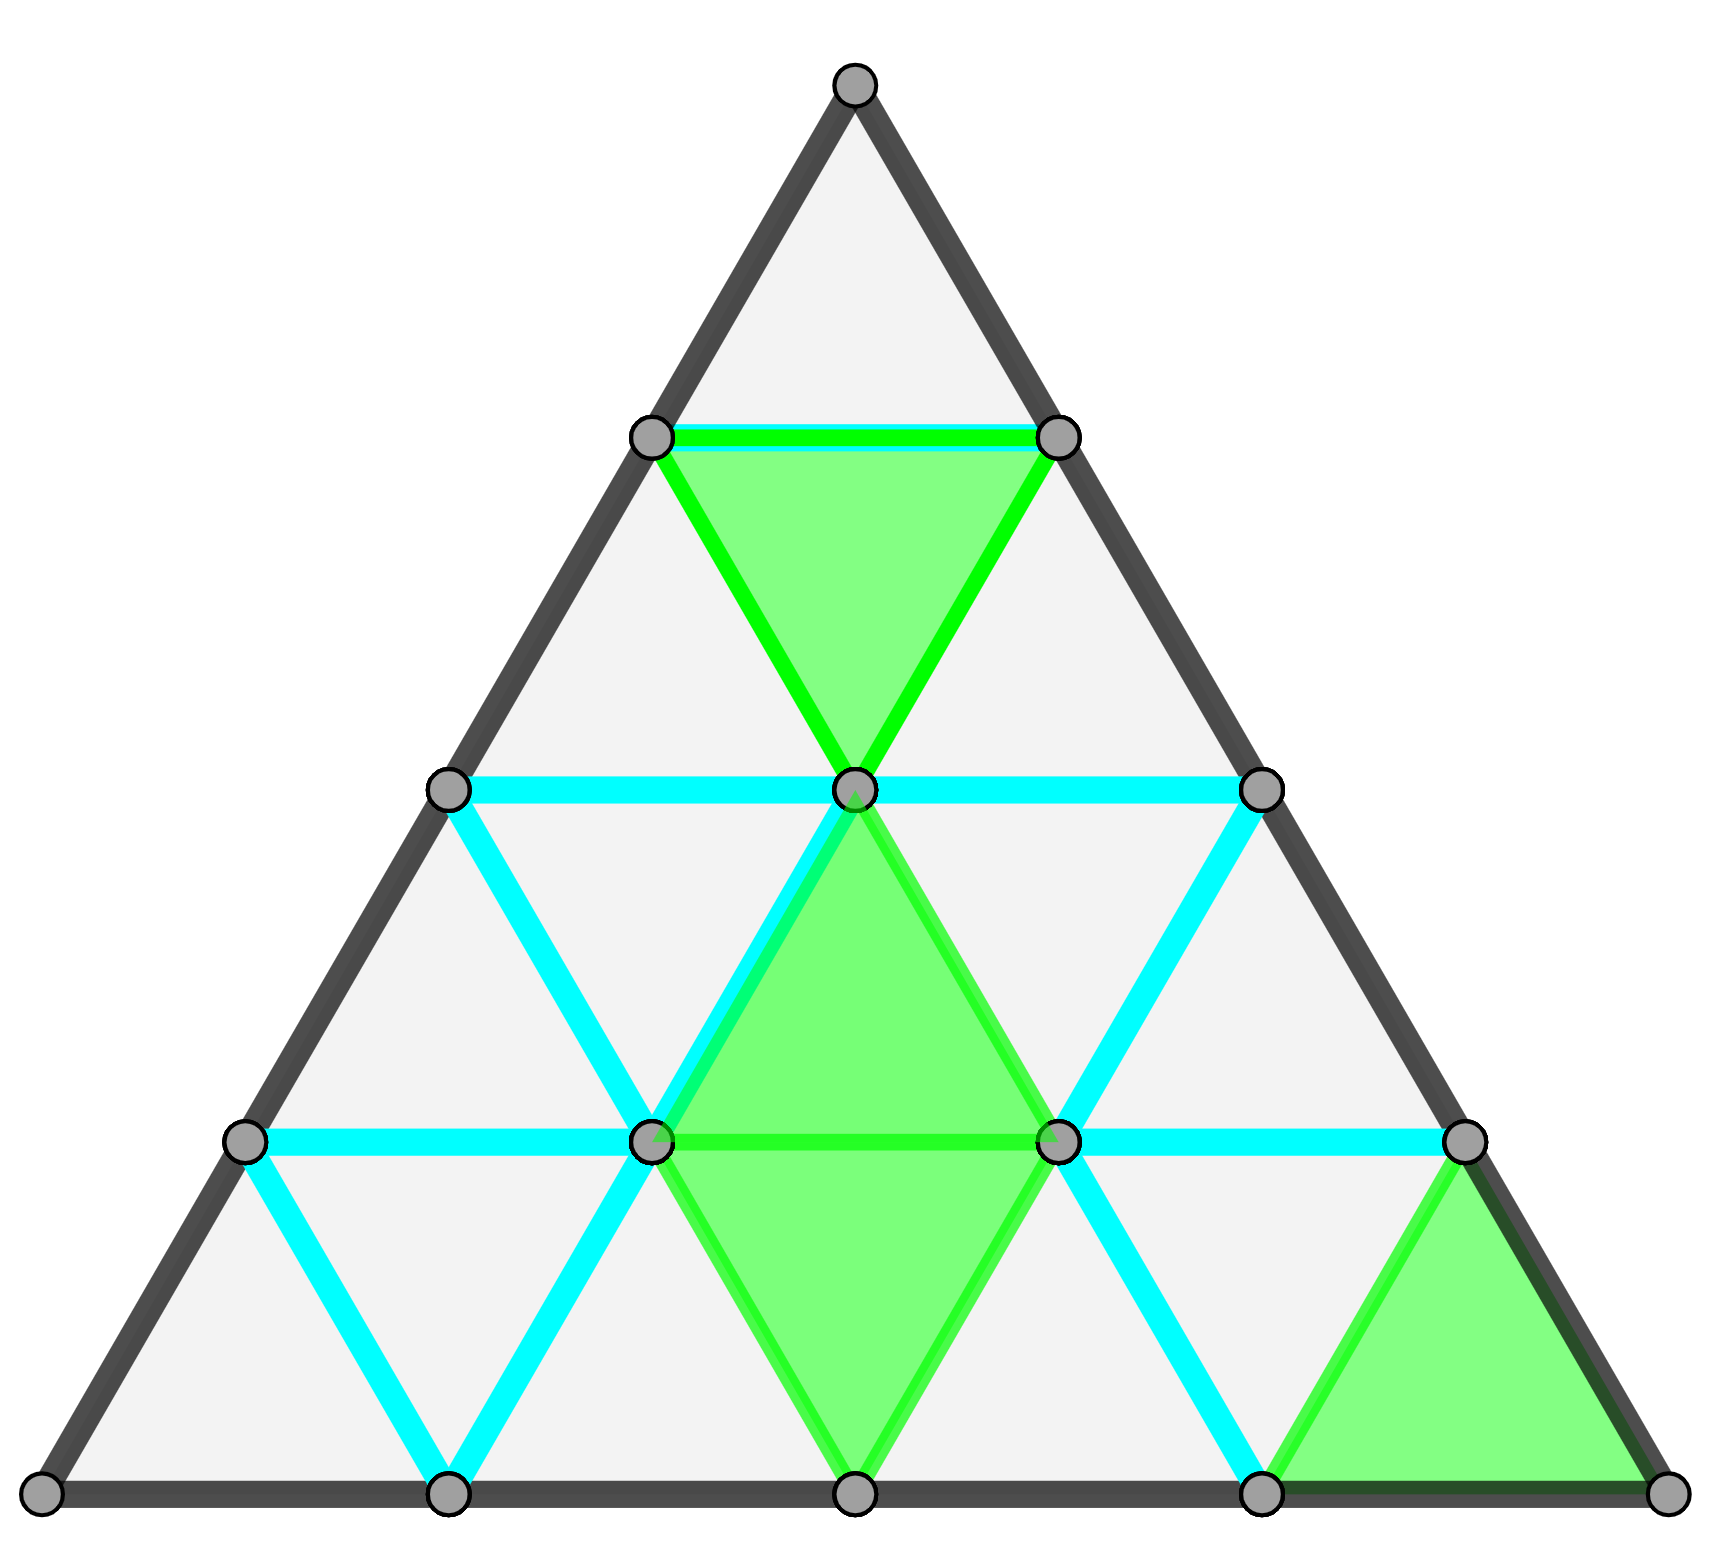
\includegraphics[width=0.35\textwidth]{image/relic2.png}
\caption{A fully charged relic after restoration. After putting 4 runestones onto the relic, all of the imprints are charged.}
\end{figure}

\newpage

Here comes the problem: What is the minimum number of energy runestones required to empower the relic fully?